% Options for packages loaded elsewhere
\PassOptionsToPackage{unicode}{hyperref}
\PassOptionsToPackage{hyphens}{url}
%
\documentclass[
]{article}
\usepackage{lmodern}
\usepackage{amssymb,amsmath}
\usepackage{ifxetex,ifluatex}
\usepackage{tikz}
\usepackage{enumerate}
\usepackage{hyperref}
\usepackage[margin=0.75in]{geometry}
\usetikzlibrary{arrows,positioning,calc}


\title{Raft Reconfig Bug (Single Node Change)}
\author{William Schultz}

\begin{document}
\maketitle

\section*{Raft Reconfig Bug Cases}

High level overview of the Raft reconfiguration bug cases laid out in Diego's \href{https://groups.google.com/g/raft-dev/c/t4xj6dJTP6E/m/d2D9LrWRza8J}{group post}. Configs are annotated with their terms i.e., a config $X$ in term $t$ is shown as $X^t$.
%
\begin{enumerate}[(1)]
    \item \textbf{One add, one remove}:
    \begin{center}
        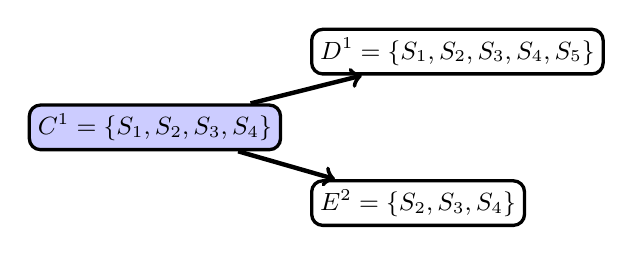
\begin{tikzpicture}
        [scale=.5,auto=left,every node/.style={circle,fill=blue!20,minimum size=1pt}]
        \small
        
        %   \node[circle, draw=black, very thick,fill=red!20] (Ca) at (0,0) {$C_{0,0}$};
        \node[rounded corners,rectangle, draw=black, very thick] (Ci)  {$C^1=\{S_1,S_2,S_3,S_4\}$};
        \node[rounded corners,rectangle, draw=black, very thick,fill=white, above right=0.5cm of Ci] (Cs)  {$D^1=\{S_1,S_2,S_3,S_4,S_5\}$};
        \node[rounded corners,rectangle, draw=black, very thick,fill=white!2,below right=0.5cm of Ci] (Cf) {$E^2=\{S_2,S_3,S_4\}$};
        % \draw (Ca) edge[->,ultra thick] (Ci);
        \draw (Ci) edge[->,ultra thick] (Cs);
        \draw (Ci) edge[->,ultra thick] (Cf);
        \end{tikzpicture}
    \end{center}

\item \textbf{Two adds}:
\begin{center}
    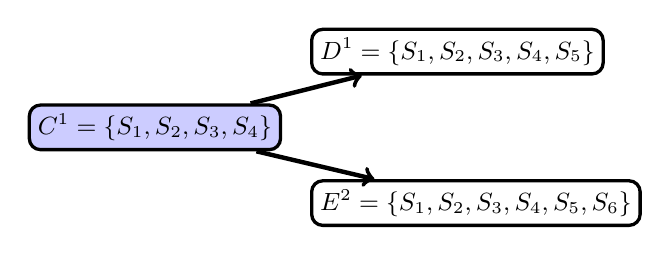
\begin{tikzpicture}
    [scale=.5,auto=left,every node/.style={circle,fill=blue!20,minimum size=1pt}]
    \small
    
    %   \node[circle, draw=black, very thick,fill=red!20] (Ca) at (0,0) {$C_{0,0}$};
    \node[rounded corners,rectangle, draw=black, very thick] (Ci)  {$C^1=\{S_1,S_2,S_3,S_4\}$};
    \node[rounded corners,rectangle, draw=black, very thick,fill=white, above right=0.5cm of Ci] (Cs)  {$D^1=\{S_1,S_2,S_3,S_4,S_5\}$};
    \node[rounded corners,rectangle, draw=black, very thick,fill=white!2,below right=0.5cm of Ci] (Cf) {$E^2=\{S_1,S_2,S_3,S_4,S_5,S_6\}$};
    % \draw (Ca) edge[->,ultra thick] (Ci);
    \draw (Ci) edge[->,ultra thick] (Cs);
    \draw (Ci) edge[->,ultra thick] (Cf);
    \end{tikzpicture}
\end{center}

\item \textbf{Two removes}:
\begin{center}
    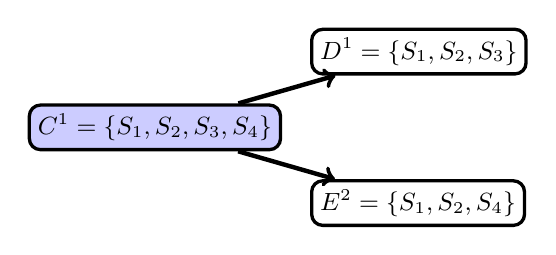
\begin{tikzpicture}
    [scale=.5,auto=left,every node/.style={circle,fill=blue!20,minimum size=1pt}]
    \small
    
    %   \node[circle, draw=black, very thick,fill=red!20] (Ca) at (0,0) {$C_{0,0}$};
    \node[rounded corners,rectangle, draw=black, very thick] (Ci)  {$C^1=\{S_1,S_2,S_3,S_4\}$};
    \node[rounded corners,rectangle, draw=black, very thick,fill=white, above right=0.5cm of Ci] (Cs)  {$D^1=\{S_1,S_2,S_3\}$};
    \node[rounded corners,rectangle, draw=black, very thick,fill=white!2,below right=0.5cm of Ci] (Cf) {$E^2=\{S_1,S_2,S_4\}$};
    % \draw (Ca) edge[->,ultra thick] (Ci);
    \draw (Ci) edge[->,ultra thick] (Cs);
    \draw (Ci) edge[->,ultra thick] (Cf);
    \end{tikzpicture}
\end{center}

\end{enumerate}

I think all of these bug cases can be viewed as instances of a common problem related to config management when logs diverge (i.e., when there are concurrent primaries in different terms). The bug arises in each case due to the fact that each child config ($D$ and $E$) has quorum overlap with its parent $C$ (due to the single node change condition), but the sibling configs don't have quorum overlap with each other. These scenarios are problematic because, for example, in case (1), config $D$ could potentially commit writes in term $1$ that are not known to leaders in config $E$ in term 2 or higher (since $D$ and $E$ don't have quorum overlap), breaking the fundamental safety property that earlier committed entries are known to newer leaders.
%
Note that this underlying problem should be avoided in joint consensus since in that case each child config will continue to contact a quorum in its parent config.

\section*{Proposed Fix}

Diego proposes the following fix:
\begin{quotation}
    The solution I'm proposing is exactly like the dissertation describes except that a leader may not append a new configuration entry until it has committed an entry from its current term.
\end{quotation}
As described above, the underlying bug can be seen as stemming from the fact that when log divergence occurs, even though each child config has quorum overlap with its parent (due to the single node change condition), the sibling configs do not necessarily have quorum overlap with each other. 

So, upon election, before doing any reconfiguration, you actually need to be sure that any \textit{sibling} configs are disabled i.e., prevented from committing writes, electing leaders, etc. You achieve this by committing a config in the parent config in your term, which disables all sibling configs in lower terms. Similarly to Diego's fix, we achieve this in MongoDB reconfig by \href{https://github.com/will62794/logless-reconfig/blob/5b1d0f3bfd93c4d78470689a56959d1dcc5297a2/MongoLoglessDynamicRaft.tla#L90-L91}{rewriting config term on primary election}, which then requires this config in the new term to become committed before further reconfigs can occur on that elected primary.

\end{document}
